\chapter{Úvod do programování a algoritmizace}
\section{Programování a algoritmizace}
Pod programováním si spousta lidí představí spoustu věcí - kdybych ale měl tento pojem popsat jednou větou, asi bych ho popsal nějak takto:

Ačkoliv né uplně přesná definice, podle mého názoru dává nejlepší představu o tom, co programování vlastně je. Programování je o hledání řešení nějakého problému, jak toto řešení vyjádřit a zajistit, aby řešení bylo co nejvhodnější danému problému. Programování už z výše uvedené definice říká, že vede k nějakému postupu, který daný problém řeší. Tento postu označujeme honosným názvem "\textbf{algoritmus}".

Nejčastěji se setkávám s přirovnáním ke kuchařce, proto si ho dovolím použít i zde: Za algoritmus můžeme považovat recept, kde máme přesnou sadu instrukcí, které nám říkají, jak něco uvařit. Tenhle recept vždy vede ke stejnému výsledku (nemůže se nám stát, že pomocí receptu na koprovku uděláme rajskou, že ano) a vždy bude doba vaření trvat stejně dlouho.

Už jenom z této intuice můžeme odvodit některé vlastnosti algoritmů:
\noindent
\begin{enumerate}
	\litem{Obecnost} Algoritmus by měl být dostatečně obecný na to, aby dokázal řešit pokud možno co nejvíce případů.
	\litem{Determinovanost} Výsledek algoritmu by měl být předvídatelný.
	\litem{Konečnost} Algoritmus musí v nějakém bodě skončit.
	\litem{Srozumitelnost} Algoritmus by měl dávat smysl a nemělo by být zbytečně složité ho pochopit.
	\litem{Efektivita} Algoritmus by neměl plýtvat zdroji a být pokud možno co nejúspornější. To samé platí i o čase potřebném na jeho vykonání.
\end{enumerate}

Tato pětice bodů je kolektivně známa jako \textbf{vlastnostni algoritmu}. Ovšem jak takový algoritmus vytvoříme? Proces takzvané \textbf{algoritmizace} by se dal popsat v následujících krocích:
\begin{enumerate}
	\litem {Analýza zadání} Pořádně se podíváme, co se po nás a našem algoritmu chce.
	\litem {Rozložení na menší problémy} Pokud je původní zadání komplexnější, rozložíme si ho na několik menších problémů, které budeme postupně řešit
	\litem {Návrh řešení} Rozmyslíme, jakými způsoby můžeme dílčí problémy řešit, a který postup by byl pro nás nejlepší.  
	\litem {Zápis algoritmu}  Algoritmus zformulujeme a zapíšeme
	\litem {Ladění} Algoritmus zkontrolujeme, zda se chová tak, jak má.
\end{enumerate}
Výsledkem této algoritmizace bude konečný sled kroků, který můžeme následně použít k vytvoření programu. Jak ale takový algoritmus zapíšeme? 

Metod je spousta, a jsou to asi takové, které by vás napadly. Můžeme algoritmus vyjádřit slovně, písemně po větách, v programovacím jazyce nebo pomocí vývojových diagramů. Hlavně poslední způsob zápisu je velmi oblíbený ve školách na otravování studentů, proto se ním tady zabývat nebudu.

Na závěr téhle kapitoly bych vám rád ukázal diagram níže, který propojuje všechny výše zmíněné pojmy dohromady a jak vlastně spolu souvisí:
\begin{figure}[H]
	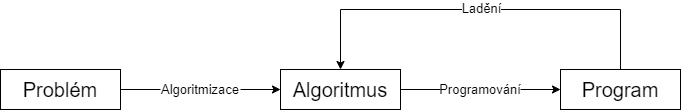
\includegraphics[width=\textwidth]{programovani_algoritmizace}
	\centering
	\caption{Diagram tvorby programu}
\end{figure}

\subsection{Asymptotická složitost algoritmů}
Vzpomeňte si zpátky na \textbf{vlastnosti algoritmu} - jednou z nich byla \textbf{efektivita}. Jak ale určíme, co je "dostatečně dobrá" efektivita, a co ne? Ačkoliv to nejde přímo univerzálně určit, protože to vždy záleží na dané situaci, ale z matematiky si můžeme vypůjčit nástroj, který nám dovolí zhruba určit, jak dlouho bude nějaká operace trvat. Tomuto nástroji se říká \textbf{asymptotická složitost} nebo také \textbf{Big O Notation}.

\begin{figure}[H]
	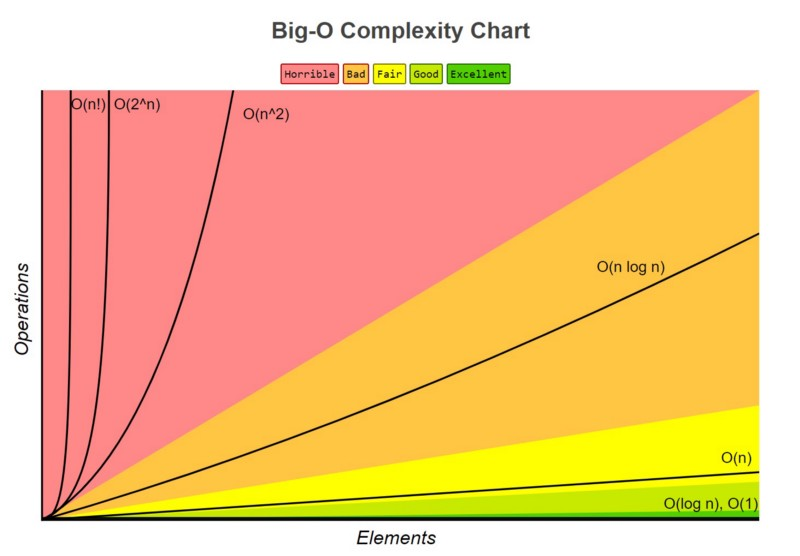
\includegraphics[width=\textwidth]{big_o_notation}
	\centering
	\caption{Graf asymptotických složitostí (freecodecamp.org)}
\end{figure}

Asymptotická složitost se určuje hlavně pro dvě domény:
\begin{enumerate}
	\litem {Časová složitost} Jak rychle roste čas potřebný na zpracování dat
	\litem {Paměťová složitost} Jak rychle roste paměť potřebná na provedení algoritmu
\end{enumerate}

Málo kdy se podaří mít optimalizovat jak čas, tak paměť (zpravidla bývá optimalizace jedné veličiny na úkor druhé). V dnešní době se spíše upřednostňuje optimalizace času, jelikož dostupné paměti je dnes docela dost.

Jak tedy takovou časovou asymptotickou složitost vypočítat? No, to je trochu složitější a je důležité říct, že je většinou spíše o odhady. Typ složitosti se dá zpravidla odhadnout z konkrétního kódu (například dvě vnořené smyčky do sebe mívají kvadratickou složitost). 

Pokud to ale nelze odhadnout, lze samozřejmě provést měření a určit jednu z funkcí, která nejlépe odpovídá nárustu v čase. Podívejte se na ilustrační obrázek níže - Na ose $x$ máme počet vstupních dat (z pravidla se používá logaritmické měřítko) a na ose $y$ čas, který byl potřeba na vykonání.

\begin{figure}[H]
	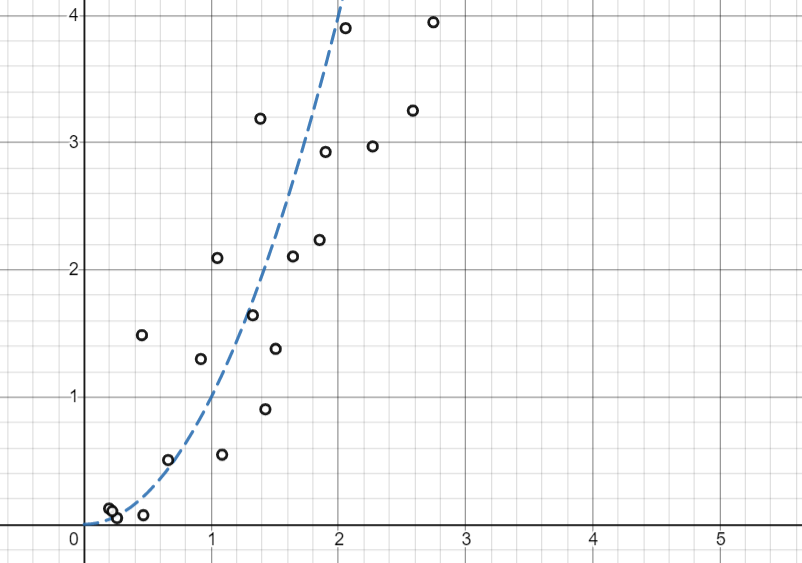
\includegraphics[width=\textwidth]{big_o_ukazka}
	\centering
	\caption{Ukázka proložení bodů z měření parabolou}
\end{figure}

Černé kroužky jsou body, které odpovídají naměřeným hodnotám, a modrá přerušovaná čára je pravá větev paraboly, kterou data prokládáme. Když se na takhle na tento obrázek podíváme, asi se shodneme, že hodnota bodů roste tak nějak podobně jako parabola, kterou jsme přidali.

S tímto závěrem bychom řekli, že funkce, která vytvářela tyhle body, má \textbf{kvadratickou časovou složitost}, nebo bychom zapsali v podobě O-notace $O(n^2)$.

Důležité si je uvědomit, že nám to neříká nic jiného, než jak čas roste v závislosti na objemu vstupních dat - nemá to být nějaký přesný výpočet - spíše jenom pomůcka k rychlému ohodnocení efektivity algoritmu.

\section{Datové typy}
Při programování pracujeme s daty různých typů - můžeme pracovat s celými čísly, reálnými čísly, s řetězci znaků a dalšími blbostmi. Datové typy programovacímu jazyku říkají, co za data chceme v proměnné ukládat, a respektive, jak je má ukládat v paměti.

Nejčastější a nejzákladnější datové typy jsou celá čísla (\textit{integers}), reálná čísla (\textit{doubles}), znaky (\textit{chars}) a textové řetězce (\textit{strings}).

Občas se ale může stát, že máme data uložena v jednom datovém typu, například řetězci znaků, a potřebujeme s ním pracovat jako s jiným typem, například číslem. To se stává často u zpracování uživatelského vstupu, který bývá celý uložen v řetězci znaků (\textit{string}) \cite{kralovcova}. Když chceme po uživateli zadat čísla, dostaneme akorát znaky, a my si musíme poradit. Pokud chceme z řetězce znaků dělat číslo, přichází na řadu proces \textbf{přetypování}.

Přetypování bývá velmi nebezpečný proces, který je často náchylný na vyvolání chyby. Proč? Představme si opět převod řetězce znaků na číslo. Při převodu mohou nastat 3 případy:
\begin{enumerate}
	\item V řetězci jsou jenom cifry, tudíž bude převod úspěšný
	\item V řetězci jsou cifry a nějaký další znak, s trochou štěstí dostameme akorát to číslo, v horším případě chybu
	\item V řetězci jsou znaky, které nelze přeložit na číslo. Buďto se vyvolá chyba, nebo se nám vrátí hodnota typu NaN.
\end{enumerate}

To jsou takové základní případy, které by mohly nastat. Může jich být více či méně, hodně záleží na samotných programovacích jazycích, jak moc se snaží běh programu zachránit. Některé při převodech chybu nevyvolají, ale pak musíme kontrolovat správnost převodu.

\section{Programovací paradigma}

Když vysvětluji, co je programovací paradigma svým kamarádům, rád říkám, že to je takový "styl programování" a přirovnávám to k zaklínačským školám z povídek Andrzeje Sapkowského (a respektive jejich videoherním adaptacím). 

Každá zaklínačská škola učí své zaklínače, jak se připravit na souboj, jak získat výhodu v boji a jak vůbec bojovat - zda být hbitý a mít výhodu rychlosti, či si držet půdu pod nohama a získat výhodu síly. Podobně je to i s programovacími paradigmaty, kde by každé paradigma odpovídalo bojovému stylu jiné zaklínačské školy.

Každé paradigma (styl) programování popisuje problém jinak, a tak vždy k výsledku dospěje jinou cestou, obecně je ale můžeme rozdělit na dvě velké kategorie:
\begin{enumerate}
	\litem{Imperativní} Zde říkáme, jaké kroky má program udělat, abychom dospěli ke chtěnému výsledku
	\litem{Deklarativní} Zde zase říkáme, co za výsledek chceme, a necháme program, ať se k němu nějak dopracuje.
\end{enumerate}

Nejčastěji se asi setkáte s jazyky \textbf{imperativními}, mezi které patří velká jména jako \textit{Java, C, C++, C\#, Rust, Python} a spousta dalších. Mezi \textbf{deklarativními} jazyky jsou také velká jména, ale jsou to jazyky spíše pro kontrolu nějakých rozhraní (například \textit{SQL} pro vytváření dotazů na databázi, či \textit{CSS} pro stylování webové stránky).

\section{Strukturované programování}

Strukturované programování je označení pro paradigma, které vzniklo z frustrace nad nestrukturovaným programováním, ve kterém bylo složité větvit program podle aktuálního stavu dat či opakovaně volat nějaký blok kódu. Ačkoliv je toto knížka o Javě, která je objektově orientovaná, připadá mi dobré zmínit základní struktury (viz tabulka \ref{table:strukturovane}), na kterých strukturované programování stojí, jelikož je objektově orientované programování v jistém slova smyslu nadstavbou ke strukturovanému.

Prvně si vysvětlíme rozdíl mezi \textbf{výrazem} a \textbf{příkazem}, a co je to \textbf{operátor}. Základním rozdílem mezi výraz a příkazem je tedy to, že výraz je vyhodnocován, a příkaz vykonáván. Operátory znáte běžně z matematiky, jedná se například o plus, mínus, krát či děleno. Operátory se ovšem ještě podle svojí funkce dají dále dělit na:

\begin{enumerate}
	\litem{Aritmetické} To jsou operátory jako $+, -, \cdot, /$
	\litem{Logické} Tyhle operátory určují logický vztah mezi levou a pravou stranou, například AND, OR, NOT, a jejich kombinace.
	\litem{Relační} Tyhle operátory určují vztah mezi hodnotami, například $<, \le, =, >, \ge$
\end{enumerate}

S výrazy, příkazy a operátory jsme nyní schopni popsat spoustu problémů. Stále zde ale máme jisté techniky a principy, které popisování problému razantně usnadňují.

\begin{table}[h!]
	\caption{Hlavní rysy strukturovaného programování}
	\label{table:strukturovane}
	\begin{tabular}{|m{0.4\linewidth} | m{0.6\linewidth} |}
		\hline
		Sekvenční zpracování instrukcí & Instrukce se vykonávají v pořadí tak, jak jsou zapsané od zhora dolů               \\ \hline
		Funkce a procedury             & Blok kódu, pomocí kterého můžeme jednou instrukcí spustit vícero vnořených příkazů \\ \hline
		Větvení programu               & Rozdělení běhu programu podle logické podmínky                                     \\ \hline
		Cykly                          & Pro opakované vykonávání instrukcí                                                 \\ \hline
	\end{tabular}
\end{table}

\section{Datové struktury}
Když se podíváme na nadpis téhle kapitoly, možná vás již napadne, že datové struktury budou něco, co nám pomůže nějakým způsobem strukturovat data. A divte se nebo ne, měli byste pravdu. Stejně jako \textbf{datové typy} říkaly, jak hodnoty ukládat v paměti, \textbf{datové struktury} nám zase říkají, jak ukládat vícero hodnot v paměti.

Tou nejprimitivnější datovou strukturou je \textbf{pole}, které najdete prakticky v každém programovacím jazyce. Pole je velmi dobré znát, jelikož díky němu dokážete vytvořit další datové struktury\footnote{Ono je to trochu složitější - lze s nimi tyto struktury vytvořit, ale né vždy budou moci konkurovat jejich nativním implementacím.}.

Pole má jednu zásadní nevýhodu, a to je jeho fixní délka. Tento problém řeší datová struktura \textbf{list} (nebo také známo jako \textbf{seznam}), jejíž délku lze libovolně rozšiřovat či zmenšovat - její nevýhodou je však větší (a tím pádem i časově náročnější) režie s pamětí\footnote{Ono ani tohle není úplně pravda - rozhodně zabírá více místa v paměti, ale pak už záleží na implemetaci (např. zřetězení prvků pomocí odkazů na další prvek má režii minimální)}.

Další obecnou datovou strukturou je \textbf{asociativní pole} (též známo jako \textbf{mapa} nebo \textbf{slovník}). Tahle struktura dále staví na konceptu \textit{pole} a rozšiřuje možnosti, jak přistupovat k prvkům. K polím přistupujeme pomocí celočíselných indexů, v asociativním poli ale můžeme používat místo celočíselného indexu takzvaný \textit{klíč}. 

Příkladem může být např. jazykový slovník, kde klíčem je cizí slovíčko, a hodnotou je český překlad. Nebo třeba telefonní seznam, kde klíčem je jméno člověka, a hodnotou je telefonní seznam\footnote{Nebo naopak. Zpravidla jsou asociativní pole jednoznačná, takže lze vytvářet inverze a z hodnot udělat klíče a naopak}.

\section{Výjimky a chybové stavy}
Bohužel nastávají situace, kdy naše programy mohou \textit{zpanikařit}. Představme si program, který se chová jako jednoduchá kalkulačka s reálnými čísly a klasickými aritmetickými operacemi. No a teď si představme, že do ní nějaký matlák\footnote{Čtěte jako matlabák} nacvaká $\frac{1}{0}$. Nulou v reálných číslech dělit neumíme, takže, co teď? Zpravidla by program takzvaně \textit{vyhodil} či \textit{vyvolal} \textbf{výjimku}. 

Výjimkou tak vyvolá například již výše zmíněné dělení nulou, nebo třeba čtení neexistujícího souboru. Výjimky jsou takto pojmenované právě kvůli tomu, že se jedná o \textit{výjimečné stavy} programu, a programovací jazyky nám dávají možnost tyto stavy ošetřit a program \textit{zotavit}. Nad výjimkou ovšem stojí ještě \textbf{chybový stav}.

Chybou může být například špatné přidělování paměti či chyba způsobená nižším rozhraním. Takovým typickým příkladem chybového stavu ze života je \textit{modrá obrazovka smrti}. Z chyb se program kvůli jejich vážnosti nezotavuje - prakticky by to ani nebylo možné.